% Prepared by Karl Ecklund September 2002
% Questions, Improvements, Comments to kme and CLEOAC
%
% LATEX 2e Template for CLEO Papers
% YOU MUST USE REVTEX4 and latex 2e
%
% Checklist for Paper Drafts:
% ---------------------------
% 0) Use appropriate \documetclass line as indicated below
% 1) Draft Number: Use latest CBX number, append A for the first vote
%                                (B,C,... for subsequent if any votes)
% 2) Don't use CLNS or CLEO numbers - this happens after your vote.
% 3) Title; use \\ to break title over several lines.
% 4) Abstract
% 5) For the Author list use CLEO Collaboration only
% 6) Body
% 
% Checklist for Journal Submissions:
% ----------------------------------
% 0) Use appropriate \documetclass line as indicated below
%    - For CLNS, hep-ex, preprints, conf. paper use CLNS version
%    - For PRL submission use PRL version
%    - For PRD submission use PRD version 
%      AND use \author{(CLEO Collaboration)} instead of \collaboration{CLEO}
%      SEE PRD_SPECIAL_CHANGEME in author list during step 5 below
% 1) CLEO paper number (from CLEOAC)
% 2) CLNS preprint number (from CLEOAC)
% 3) Title; use \\ to break title over several lines.
% 4) Abstract
% 5) Author list (from CLEOAC)
% 6) PACS codes
% 7) Body
% 8) Add acknowledgments
% 9) Hardcode the \date when ready to submit to journal and hep-ex.
%
% Checklist for Conference Papers:
% --------------------------------
% 0) Use appropriate \documetclass line as indicated below
%    - For conf. paper use CLNS version
% 1) CLEO conference paper number (from CLEOAC) (don't use CLNS)
% 2) Title; use \\ to break title over several lines.
% 3) To \thanks after title, add appropriate conference info.
% 4) Abstract
% 5) Author list (from CLEOAC)
% 6) Body
% 7) Add acknowledgments
% 8) Hardcode the \date when ready to submit to conference and hep-ex.
% 
% KNOWN PROBLEMS with template and REVTEX4
% - can't have \collaboration in PRD style grouped author list
%   Using \author{(CLEO Collaboration)} instead
% - can't make abstract appear before full author list ala CLNS notes
%   Abandoning this as the format for CLNS.

%%%%%%%%%%%%%%%%%%%%%%%%%%%%%%%%%%%%%%%%%%%%%%%%%%%%%%%%%%%%%%%%%%%%%%
% Select one of the \documentclass lines below for your paper
%%%%%%%%%%%%%%%%%%%%%%%%%%%%%%%%%%%%%%%%%%%%%%%%%%%%%%%%%%%%%%%%%%%%%%
%%%%%%%%%%%%%% Use for CLNS preprint (hep-ex) and Paper Drafts
\documentclass[aps,prd,preprint,superscriptaddress,tightenlines,nofootinbib,floatfix]{revtex4}

%%%%%%%%%%%%%% Use for PRL
%\documentclass[aps,prl,twocolumn,superscriptaddress,showpacs]{revtex4}

%%%%%%%%%%%%%% Use for PRD submission
%\documentclass[aps,prd,preprint,nopreprintnumbers,nofootinbib,showpacs]{revtex4}
%%%%%%%%%%%%%% Use for PRD formatting tables and figures in 2 column
%\documentclass[aps,prd,twocolumn,nofootinbib,showpacs]{revtex4}

\usepackage{graphicx}% Include figure files
\usepackage{dcolumn}% Align table columns on decimal point
\usepackage{bm}% bold math
\usepackage{multirow}% multirow table entries
\usepackage{amsmath}

\begin{document}

%-Definitions-----------------------------------------------------------
\newcommand{\barb}{\bar{B}}
%\newcommand{\bbbar}{B\bar{B}}
%\newcommand{\bm}{B^-}
\newcommand{\bob}{\bar{B}^0}
\newcommand{\bo}{B^0}
\newcommand{\bp}{B^+}
\newcommand{\dkpipiz}{D^0 \to K^-\pi^+\pi^0}
\newcommand{\dkpi}{D^0 \to K^-\pi^+}
\newcommand{\dkrho}{D^0 \to K^- \rho^+}
\newcommand{\dobar}{\overline{D}^0}
\newcommand{\etal}{{\it et al.}}
\newcommand{\F}{$\cal F$}
%\newcommand{\gev}{\ \rm GeV}
\newcommand{\kpipiz}{K^-\pi^+\pi^0}
%\newcommand{\kpi}{K^-\pi^+}
\newcommand{\krho}{K^- \rho^+}
%\newcommand{\mev}{\ \rm MeV}
\newcommand{\piz}{\pi^0}
\newcommand{\ra}{{\rightarrow}}
\newcommand{\Ufs}{\Upsilon(4S)}

\newcommand{\about}		{\mbox{$\sim$}}
\newcommand{\aerr}[3]   {\mbox{${{#1}^{+ #2}_{- #3}}$}}
\newcommand{\amp}    	{\mbox{${\cal A}$}}
\newcommand{\avcb}		{\mbox{$|V_{cb}|$}}
\newcommand{\avtb}		{\mbox{$|V_{tb}|$}}
\newcommand{\avtd}		{\mbox{$|V_{td}|$}}
\newcommand{\avts}		{\mbox{$|V_{ts}|$}}
\newcommand{\avub}		{\mbox{$|V_{ub}|$}}
\newcommand{\avud}		{\mbox{$|V_{ud}|$}}
\newcommand{\avus}		{\mbox{$|V_{us}|$}}
\newcommand{\BBbar}     {\mbox{$B\bar B$}}
\newcommand{\bbbar}     {\mbox{$B\bar B$}}
\newcommand{\bc}		{\mbox{$b\to c$}}
\newcommand{\bdb}		{\mbox{$\bar B^0_d $}}
\newcommand{\bd}		{\mbox{$B^0_d $}}
\newcommand{\berr}[2]   {\mbox{${{}^{+ #1}_{- #2}}$}}
\newcommand{\bmeson}	{\mbox{$B$}}
\newcommand{\bqb}		{\mbox{$\bar B^0_q $}}
\newcommand{\bq}		{\mbox{$B^0_q $}}
\newcommand{\branch}    {\mbox{${\cal B}$}}
\newcommand{\bsb}		{\mbox{$\bar B^0_s$}}
\newcommand{\bs}		{\mbox{$B^0_s$}}
\newcommand{\bu}		{\mbox{$b\to u$}}
\newcommand{\cerr}[4]   {\mbox{${{}^{+ #1}_{- #2}{}^{+ #3}_{- #4}}$}}
\newcommand{\chisq}		{\mbox{$\chi^2$}}
\newcommand{\cosB}		{\mbox{${\cos\theta_{\rm B}}$}}
\newcommand{\cossph}	{\mbox{$\cos \theta_{\rm sph}$}}
\newcommand{\costhr}	{\mbox{$\cos \theta_{\rm thr}$}}
\newcommand{\dedx}		{\mbox{$dE/dx$}}
\newcommand{\derr}[5]   {\mbox{${{#1}^{+ #2}_{- #3}{}^{+ #4}_{- #5}}$}}
\newcommand{\de}		{\mbox{$\Delta E$}}
\newcommand{\dzerobar}	{\mbox{$\overline {D^0}$}}
\newcommand{\dzero}		{\mbox{${D^0}$}}
\newcommand{\ebeam}		{\mbox{$E_{\rm beam}$}}
\newcommand{\eb}		{\mbox{$E_b$}}
\newcommand{\eeqq}		{\mbox{$e^+e^-\to\qqb$}}
\newcommand{\ee}		{\mbox{$e^+e^-$}}
%\newcommand{\etal}		{\mbox{${\it et al}$}}
\newcommand{\expt}		{\mbox{$_{\rm expt}$}}
\newcommand{\fbinv}		{\mbox{${\rm fb}^{-1}$}}
%\newcommand{\fisher}    {\mbox{${\cal F}$}}
\newcommand{\fisher}    {\mbox{$x_{\cal F}$}}
\newcommand{\gev}		{\mbox{${\rm ~GeV}$}}
\newcommand{\hh}		{\mbox{$h^+h^-$}}
\newcommand{\hpm}		{\mbox{$h^\pm$}}
%\newcommand{\implies}	{\mbox{${\Longrightarrow}$}}
\newcommand{\jimexp}[1]	{\mbox{${\rm e}^{{#1}}$}}
\newcommand{\kk}		{\mbox{KK}}
\newcommand{\Kpi}		{\mbox{$K\pi$}}
\newcommand{\kpi}		{\mbox{$\Kpi$}}
\newcommand{\kpz}		{\mbox{$K^+\pi^0$}}
\newcommand{\KP}		{\mbox{$K\pi$}}
\newcommand{\ksp}		{\mbox{$K^0_S\pi^+$}}
\newcommand{\ks}		{\mbox{$K^0_S$}}
\newcommand{\kz}		{\mbox{$K^0$}}
\newcommand{\kzb}		{\mbox{$\overline{K^0}$}}
\newcommand{\like}    	{\mbox{${\cal L}$}}
\newcommand{\Lp}		{\mbox{$\Lambda \bar p$}}
\newcommand{\lum}    	{\mbox{${\cal L}$}}
\newcommand{\mb}		{\mbox{$M_B$}}
\newcommand{\mev}		{\mbox{${\rm MeV}$}}
\newcommand{\micron}	{\mbox{$~\mu{\rm m}$}}
\newcommand{\mm}		{\mbox{$\mu^+\mu^-$}}
\newcommand{\model}		{\mbox{$_{\rm mod}$}}
\newcommand{\nbb}		{\mbox{$N_{B\bar B}$}}
\newcommand{\nbinv}		{\mbox{${\rm nb}^{-1}$}}
\newcommand{\pb}        {\mbox{$p_B$}}
\newcommand{\pbinv}		{\mbox{${\rm pb}^{-1}$}}
\newcommand{\pdf}		{\mbox{${PDF}$}}
\newcommand{\pdfs}		{\mbox{${PDF}{\rm s}$}}
\newcommand{\pidkpi}	{\mbox{$\Delta_{K\pi}$}}
\newcommand{\pidkp}		{\mbox{$\Delta_{Kp}$}}
\newcommand{\pid}		{\mbox{$\Delta_{PID}$}}
\newcommand{\pipi}		{\mbox{$\Pipi$}}
\newcommand{\Pipi}		{\mbox{$\pi\pi$}}
\newcommand{\power}[1]  {\mbox{${\times 10^{#1}}$}}
\newcommand{\ppz}		{\mbox{$\pi^+\pi^0$}}
\newcommand{\pvec}		{\mbox{$\vec{p}$}}
\newcommand{\pz}		{\mbox{$\pi^0$}}
\newcommand{\qqb}		{\mbox{$q\bar q$}}
\newcommand{\qq}		{\mbox{${q\bar q}$}}
\newcommand{\stat}		{\mbox{$_{\rm stat}$}}
\newcommand{\syst}		{\mbox{$_{\rm syst}$}}
\newcommand{\theo}		{\mbox{$_{\rm theo}$}}
\newcommand{\upsi}		{\mbox{$\Upsilon$({\rm 4S})}}
\newcommand{\vcb}		{\mbox{$V_{cb}$}}
\newcommand{\vcd}		{\mbox{$V_{cd}$}}
\newcommand{\vcs}		{\mbox{$V_{cs}$}}
\newcommand{\vtb}		{\mbox{$V_{tb}$}}
\newcommand{\vtd}		{\mbox{$V_{td}$}}
\newcommand{\vts}		{\mbox{$V_{ts}$}}
\newcommand{\vub}		{\mbox{$V_{ub}$}}
\newcommand{\vud}		{\mbox{$V_{ud}$}}
\newcommand{\vus}		{\mbox{$V_{us}$}}
\newcommand{\zhat}		{\mbox{$\hat{\bf z}$}}

\newcommand{\ppbar}		{\mbox{${p\bar p}$}}
\newcommand{\pL}		{\mbox{${p\bar\Lambda}$}}
\newcommand{\LL}		{\mbox{${\Lambda\bar\Lambda}$}}

\newcommand{\mpdf}    	{\mbox{${\cal M}$}}
\newcommand{\epdf}    	{\mbox{${\cal E}$}}
\newcommand{\fpdf}    	{\mbox{${\cal F}$}}
\newcommand{\cpdf}    	{\mbox{${\cal C}$}}
\newcommand{\dkmode}	{\mbox{${\mu}$}}
\newcommand{\contrib}	{\mbox{${\kappa}$}}
\newcommand{\mc}    	{\mbox{${}_{\dkmode\contrib}$}}
\newcommand{\nk}    	{\mbox{${n}_{\contrib}$}}

\newcommand{\G}		{\mbox{${G}$}}
\newcommand{\GG}	{\mbox{${\cal G}$}}
\newcommand{\ARG}	{\mbox{${A}$}}
\newcommand{\LIN}	{\mbox{${L}$}}
\newcommand{\BW}	{\mbox{${\cal R}$}}
\newcommand{\FI}	{\mbox{${F_0}$}}
\newcommand{\DG}	{\mbox{${a\G_1+b\G_2}$}}
\newcommand{\GGG}	{\mbox{${a\G+b\GG}$}}
\newcommand{\DGG}	{\mbox{${a\GG_1+b\GG_2}$}}

\newcommand{\sba} 	{\mbox{${S/B}$}}
\newcommand{\rfw}   {\mbox{$R_2$}}
\newcommand{\effmc}     {\mbox{${\epsilon_{\rm MC}}$}}
\newcommand{\effdata}     {\mbox{${\epsilon_{\rm DATA}}$}}

\newcommand{\RR}	{\mbox{${\cal R}$}}

\newcommand{\subs}[1]{{\mbox{\scriptsize #1}}}
\newcommand{\re}{\mathrm{Re\:}}
\newcommand{\gee}{$\Gamma_{ee}$}
\newcommand{\ups}{$\Upsilon$}
\newcommand{\uone}{$\Upsilon(1S)$}
\newcommand{\utwo}{$\Upsilon(2S)$}
\newcommand{\uthree}{$\Upsilon(3S)$}
\newcommand{\mpprec}{$m_\subs{$\pi\pi$-rec}$}
\newcommand{\bbar}{$b\bar{b}$}
\newcommand{\inv}{$^{-1}$}
\newcommand{\twotoone}{$\Upsilon(2S) \to \pi^+\pi^- \Upsilon(1S)$}
\newcommand{\pip}{$\pi^+\pi^-$}
\newcommand{\tautau}{$\tau^+\tau^-$}
\newcommand{\dxy}{$d_{XY}$}
\newcommand{\dz}{$d_Z$}

%-----------------------------------------------------------------------
%-----------------------------------------------------------------------
%-----------------------------------------------------------------------

%\preprint line(s) will be ignored for PRL/PRD
%\preprint{CLEO Draft YY-NNA} % For paper draft CBX YY-NN -> Draft YY-NNA
%\preprint{CLEO CONF YY-NN}   % For conference papers
%\preprint{ICHEP ABSnnn}      % For conference papers
\preprint{CLNS 05/XXXX; CLEO 05-XX}       % for CLNS notes
\preprint{EPS-XXX}         % for CLNS notes

\title{Di-electron Widths of the Upsilon(1S,2S,3S) Resonances}

\thanks{Archived as hep-ex/XXXXXXX; 
submitted to {\it Phys. Rev. Q}}

%-------- INSERT HERE ------------
% Your author list goes here  REMOVE EVERYTHING to END INSERT and
% replace with your authorlist (ask cleoac).


\author{A.~Bornheim}
\author{E.~Lipeles}
\author{S.~P.~Pappas}
\author{A.~Shapiro}
\author{W.~M.~Sun}
\author{A.~J.~Weinstein}
\affiliation{California Institute of Technology, Pasadena, California 91125}
\author{R.~A.~Briere}
\author{G.~P.~Chen}
\author{T.~Ferguson}
\author{G.~Tatishvili}
\author{H.~Vogel}
\affiliation{Carnegie Mellon University, Pittsburgh, Pennsylvania 15213}
\author{N.~E.~Adam}
\author{J.~P.~Alexander}
\author{K.~Berkelman}
\author{F.~Blanc}
\author{V.~Boisvert}
\author{D.~G.~Cassel}
\author{P.~S.~Drell}
\author{J.~E.~Duboscq}
\author{K.~M.~Ecklund}
\author{R.~Ehrlich}
\author{R.~S.~Galik}
\author{L.~Gibbons}
\author{B.~Gittelman}
\author{S.~W.~Gray}
\author{D.~L.~Hartill}
\author{B.~K.~Heltsley}
\author{L.~Hsu}
\author{C.~D.~Jones}
\author{J.~Kandaswamy}
\author{D.~L.~Kreinick}
\author{A.~Magerkurth}
\author{H.~Mahlke-Kr\"uger}
\author{T.~O.~Meyer}
\author{N.~B.~Mistry}
\author{J.~R.~Patterson}
\author{D.~Peterson}
\author{J.~Pivarski}
\author{S.~J.~Richichi}
\author{D.~Riley}
\author{A.~J.~Sadoff}
\author{H.~Schwarthoff}
\author{M.~R.~Shepherd}
\author{J.~G.~Thayer}
\author{D.~Urner}
\author{T.~Wilksen}
\author{A.~Warburton}
\author{M.~Weinberger}
\affiliation{Cornell University, Ithaca, New York 14853}
\author{S.~B.~Athar}
\author{P.~Avery}
\author{L.~Breva-Newell}
\author{V.~Potlia}
\author{H.~Stoeck}
\author{J.~Yelton}
\affiliation{University of Florida, Gainesville, Florida 32611}
\author{K.~Benslama}
\author{B.~I.~Eisenstein}
\author{G.~D.~Gollin}
\author{I.~Karliner}
\author{N.~Lowrey}
\author{C.~Plager}
\author{C.~Sedlack}
\author{M.~Selen}
\author{J.~J.~Thaler}
\author{J.~Williams}
\affiliation{University of Illinois, Urbana-Champaign, Illinois 61801}
\author{K.~W.~Edwards}
\affiliation{Carleton University, Ottawa, Ontario, Canada K1S 5B6 \\
and the Institute of Particle Physics, Canada M5S 1A7}
\author{D.~Besson}
\author{X.~Zhao}
\affiliation{University of Kansas, Lawrence, Kansas 66045}
\author{S.~Anderson}
\author{V.~V.~Frolov}
\author{D.~T.~Gong}
\author{Y.~Kubota}
\author{S.~Z.~Li}
\author{R.~Poling}
\author{A.~Smith}
\author{C.~J.~Stepaniak}
\author{J.~Urheim}
\affiliation{University of Minnesota, Minneapolis, Minnesota 55455}
\author{Z.~Metreveli}
\author{K.K.~Seth}
\author{A.~Tomaradze}
\author{P.~Zweber}
\affiliation{Northwestern University, Evanston, Illinois 60208}
\author{S.~Ahmed}
\author{M.~S.~Alam}
\author{J.~Ernst}
\author{L.~Jian}
\author{M.~Saleem}
\author{F.~Wappler}
\affiliation{State University of New York at Albany, Albany, New York 12222}
\author{K.~Arms}
\author{E.~Eckhart}
\author{K.~K.~Gan}
\author{C.~Gwon}
\author{K.~Honscheid}
\author{D.~Hufnagel}
\author{H.~Kagan}
\author{R.~Kass}
\author{T.~K.~Pedlar}
\author{E.~von~Toerne}
\author{M.~M.~Zoeller}
\affiliation{Ohio State University, Columbus, Ohio 43210}
\author{H.~Severini}
\author{P.~Skubic}
\affiliation{University of Oklahoma, Norman, Oklahoma 73019}
\author{S.A.~Dytman}
\author{J.A.~Mueller}
\author{S.~Nam}
\author{V.~Savinov}
\affiliation{University of Pittsburgh, Pittsburgh, Pennsylvania 15260}
\author{J.~W.~Hinson}
\author{J.~Lee}
\author{D.~H.~Miller}
\author{V.~Pavlunin}
\author{B.~Sanghi}
\author{E.~I.~Shibata}
\author{I.~P.~J.~Shipsey}
\affiliation{Purdue University, West Lafayette, Indiana 47907}
\author{D.~Cronin-Hennessy}
\author{A.L.~Lyon}
\author{C.~S.~Park}
\author{W.~Park}
\author{J.~B.~Thayer}
\author{E.~H.~Thorndike}
\affiliation{University of Rochester, Rochester, New York 14627}
\author{T.~E.~Coan}
\author{Y.~S.~Gao}
\author{F.~Liu}
\author{Y.~Maravin}
\author{R.~Stroynowski}
\affiliation{Southern Methodist University, Dallas, Texas 75275}
\author{M.~Artuso}
\author{C.~Boulahouache}
\author{S.~Blusk}
\author{K.~Bukin}
\author{E.~Dambasuren}
\author{R.~Mountain}
\author{H.~Muramatsu}
\author{R.~Nandakumar}
\author{T.~Skwarnicki}
\author{S.~Stone}
\author{J.C.~Wang}
\affiliation{Syracuse University, Syracuse, New York 13244}
\author{A.~H.~Mahmood}
\affiliation{University of Texas - Pan American, Edinburg, Texas 78539}
\author{S.~E.~Csorna}
\author{I.~Danko}
\affiliation{Vanderbilt University, Nashville, Tennessee 37235}
\author{G.~Bonvicini}
\author{D.~Cinabro}
\author{M.~Dubrovin}
\author{S.~McGee}
\affiliation{Wayne State University, Detroit, Michigan 48202}
%\author{(CLEO Collaboration)} %FOR PRD_SPECIAL_CHANGEME
\collaboration{CLEO Collaboration} %FOR PRL,CLNS
\noaffiliation

%\author{John Doe}
%\affiliation{Physics Department, Cornell University
%Ithaca, New York 14853}
%\author{(CLEO Collaboration)}     %FOR PRD_SPECIAL_CHANGEME
%\collaboration{CLEO Collaboration} %FOR PRL and CLNS (superscriptaddress)
%\noaffiliation

%-------- END INSERT ------------

%please hard code the date when you have a final draft and submit to CLEOAC
\date{\today}



%---------------------------------------------------------------------
%
%\abstract
%
%---------------------------------------------------------------------

\begin{abstract} 
We have determined the di-electron widths (\gee) of the \uone, \utwo,
and \uthree\ from the integrated production cross section of each
resonance in \ee\ collisions.  To measure these widths to a
few-percent precision, the Cornell Electron Storage Ring (CESR)
scanned the lineshapes of the three resonances, providing the CLEO
detector with a total of 0.26 fb\inv\ of lineshape scan data, and an
additional 2.2 fb\inv\ at the resonance peaks and continuum below each
peak.  We present the results of these measurements, which are a
precise check on lattice QCD calculations for an observable related to
$f_B$.
\end{abstract}
\pacs{13.20.He}
\maketitle

%---------------------------------------------------------------------
%
\section{Introduction}
%
%---------------------------------------------------------------------

\begin{figure}[t]
  \begin{center}
    \includegraphics[width=0.9\linewidth]{../plots/proceedings_diagrams}
  \end{center}
  \caption{\label{fig:diagrams} Feynman diagrams for (a) the process
  measured by \gee, (b) the process measured by $f_B$.}
\end{figure}

The di-electron width, \gee, of \uone, \utwo, and \uthree\ measures
the coupling of the \ups\ \bbar\ resonance to a two-electron state.
In the absence of other \ups\ decays, \gee\ would be the inverse
lifetime of the \ups\ and the full-width at half-maximum of the \ups's
rest mass distribution.  Since \ups\ does decay to other final states,
$\Gamma_{ee} = \mathcal{B}_{ee} \Gamma$, and represents about 1 keV of
the \ups's 50 keV full width.  Given $\mathcal{B}_{ee}$, \gee\ is used
to determine $\Gamma$.

The $\Upsilon \to e^+e^-$ process consists of two steps: first the two
$b$ quarks must find each other and annihilate, then \ee\ are produced
electromagnetically through a virtual photon (see Figure
\ref{fig:diagrams}-a).  This second step is well-understood QED, and
can be used as a probe of the QCD involve in the first.  For instance,
the \bbar\ spacial wavefunction, evaluated at the origin, can be
calculated as
\begin{equation}
  |\psi(0,0,0)|^2 = \left(\frac{3 {M_\Upsilon}^2}{16 \pi
   {\alpha_\subs{QED}}^2} \right) \Gamma_{ee}
\end{equation}
because the two $b$ quarks must fluctuate to the same point in space
before annihilation.  This gives us some idea of the width of the
wavefunction in space, and therefore the strength of the force that
binds the two quarks.

Most importantly, \gee\ can test the newly ``unquenched'' lattice
calculations \cite{davies} because it can be calculated to high
accuracy (2--5\%).  This anticipated theoretical accuracy is better
than the current experimental precision of \gee\ (for the \utwo\ and
\uthree\ at least), so a new set of high-precision measurements would
test the predictive power of the unquenched techniques.  Also, notice
the similarity of the process measured by \gee\ and that of $f_B$
(Figure \ref{fig:diagrams}): the QCD part differs only in the mass of
one quark in a central force problem.  Verification of the lattice
\gee\ calculation would lend credence to a lattice $f_B$ calculation.

%---------------------------------------------------------------------
%
\section{Measurement Technique, Datasets, and Detector}
%
%---------------------------------------------------------------------

Perhaps surprisingly, \gee\ is not measured by observing $\Upsilon \to
e^+e^-$, but by observing $e^+e^- \to \Upsilon$.  This is because the
50 keV full width is too narrow to be measured directly, and $\Upsilon
\to e^+e^-$ can only be used to get $\mathcal{B}_{ee}$.  The
production process, $e^+e^- \to \Upsilon$, is related to the decay by
crossing symmetry, provided we integrate over initial-state \ee\
energies.
\begin{equation}
  \Gamma_{ee} = \frac{6\pi^2}{M_\Upsilon} \int \sigma(e^+e^- \to
  \Upsilon) \, dE, \label{eqn:geesig}
\end{equation}
where $\sigma$ is the production cross-section.

We measure the \ups\ production cross-section at the Cornell Electron
Storage Ring (CESR) as a function of incident beam energy (a tunable
parameter), and call this distribution the lineshape.  (It is a
spectral line in analogy with the short-lived excited states of
Hydrogen.)  The area under this lineshape, if it were a pure
Breit-Wigner resonance, is the integral needed by Equation
\ref{eqn:geesig}.  The energy spread of the \ee\ is about 4 MeV in
CESR, and this convolves the Breit-Wigner with a Gaussian that
obscures its natural width but preserves its area exactly.  Another
complication is that high-energy \ee\ beams can radiate a photon
before colliding, reducing their energy to the \ups\ mass, and then
produce an \ups\ state.  This raises the cross-section on the
high-energy side of the resonance peak.  This (divergent) high-energy
tail should not be included in the integral, so \gee\ is measured by
fitting the observed lineshape to a three-way convolution of
Breit-Wigner, Gaussian, and initial-state radiation tail (calculated
by Kuriev and Fadin \cite{kf}) with the Breit-Wigner area as a
floating parameter (see Figure \ref{fig:cartoon}).

\begin{figure}[t]
  \begin{center}
    \includegraphics[width=0.6\linewidth]{../plots/proceedings_cartoon}
  \end{center}
  \caption{\label{fig:cartoon} A cartoon of the \gee\ measurement: we
    observe the shape of the Breit-Wigner, Gaussian, ISR tail
    convolution in cross-section versus beam energy and fit for the
    area of the Breit-Wigner.}
\end{figure}

CESR devoted 0.10 fb\inv, 0.06 fb\inv, and 0.10 fb\inv\ to scans of
the \uone, \utwo, and \uthree\ lineshapes between November 2001 and
August 2002.  Each resonance was scanned once a week, and each
weekly scan covered the entire resonance to be able to act as an
independent measurement of \gee.  This is because we were afraid that
the beam energy measurement would lose its calibration from one scan
to the next: the beam energy is measured with an NMR probe in a test
magnet in series with the ring magnets, and it may be displaced by
machine studies between scans.

In addition to the dedicated scan data, we included general-purpose
off-resonance and on-resonance data as points in the lineshape.
Off-resonance data were collected about 20 MeV below each resonance
(0.18 fb\inv, 0.44 fb\inv, and 0.16 fb\inv), which is far enough from
the resonance that they are insensitive to weekly shifts in beam
energy.  These data have been combined into a single cross-section
measurement.  On-resonance data are sensitive to beam energy
differences, so only data not separated from a scan by machine studies
are used (0.60 fb\inv, 0.10 fb\inv, 0.71 fb\inv).

The \ups\ cross-section was measured at each energy point by CLEO, a
nearly $4\pi$ general-purpose detector built around the CESR collision
point.  This analysis only made use of the central drift chamber and
inner silicon vertex detector for charged particle tracking (in a
solenoidal magnetic field) and the CsI crystal calorimeter for
measuring the energies and trajectories of neutral particles.  The
CLEO trigger accepts events that have a minimum number of trigger
tracks (AXIAL if observed in the first 16 drift chamber layers, STEREO
if extended into the remaining 31) and calorimeter clusters (CBLO if a
calorimeter tile measures more than 150 MeV, CBMD if 750 MeV, and CBHI
if 1.5 GeV).  Our analysis trigger accepts events with at least
\begin{multline}
  \mbox{(3 AXIAL and 1 CBLO) or} \\
  \mbox{(2 STEREO and (2 CBLO or 1 CBMD)) or} \\
  \mbox{(1 AXIAL and 1 CBMD).} \label{eqn:trig}
\end{multline}
We will also make use of a prescaled two-track trigger (2 AXIAL and
5\% probability) and a Gamgam trigger (2 CBHI on opposite sides of the
calorimeter barrel) for $e^+e^- \to \gamma\gamma$.

CLEO data were taken in one-hour runs that correspond to fills of the
electron storage ring.  About 2\% of the relevant runs were excluded
because of trigger and event selection inefficiencies peculiar to
these runs.

%---------------------------------------------------------------------
%
\section{Cross-section Measurement}
%
%---------------------------------------------------------------------

The central objective of this analysis is to produce a plot of \ups\
cross-section versus energy, which can be fitted for \gee.  We will
first establish a set of cuts, selection criteria which define a
sample of \ups\ decays, and estimate the number of false positives in
this sample.  Having subtracted these backgrounds from our \ups\
count, we will then consider the inverse problem: how many \ups\
events were left out.  This can be determined directly for \uone\
events, as the decay \twotoone\ provides two charged tracks (\pip)
which can be used to identify the event with little ambiguity.  From
this second, unbiased sample, we count the fraction of \uone\ events
which satisfy our cuts, thus measuring the cuts' efficiency for \uone\
decays without theoretical prejudice.  The more energetic states,
\utwo\ and \uthree, can decay the same ways as the \uone, but can
additionally cascade to lower-energy \bbar\ bound states (such as
\uone\ or $\chi_b(1P)$) before the $b$ quarks annihilate.  This adds a
correction to the \utwo\ and \uthree\ efficiencies, but it is
well-understood and can be simulated with Monte Carlo.

Then we will have a true number of $e^+e^- \to \Upsilon$ events, but
this is a function of the luminosity (overlap and focus) of the \ee\
beams and the length of time we collected data.  To translate this to
a cross-section that could be measured by any \ee\ collider, we need
to divide out these machine-dependent parameters.  This factor, the
integrated luminosity, is determined by counting a subset of Gamgam
($e^+e^- \to \gamma\gamma$) events and comparing them with a
theoretical prediction of their rate for a given luminosity.  The
$e^+e^- \to \Upsilon$ cross-section in the same data-taking period is
\begin{equation}
  \sigma_{e^+e^- \to \Upsilon} \mbox{ (nb)} = \frac{\#(e^+e^- \to
  \Upsilon)}{\#(e^+e^- \to \gamma\gamma)} \, \times \, \frac{\mbox{predicted }
  \#(e^+e^- \to \gamma\gamma)}{\mbox{given luminosity (nb\inv)}}
\end{equation}
The Gamgam event type was chosen as the measure of luminosity because
it is a well-understood QED process and has negligible background from
\ups\ decays, as $\Upsilon$ and $\gamma\gamma$ have incompatible
angular momenta.

%---------------------------------------------------------------------
%
\subsection{Selection Criteria and Backgrounds} \label{sec:back}
%
%---------------------------------------------------------------------

To suppress large continuum backgrounds such as Bhabhas ($e^+e^- \to
e^+e^-$), we select only hadronic events, that is, all \ups\ decays
except $\Upsilon \to e^+e^-$, $\Upsilon \to \mu^+\mu^-$, and $\Upsilon
\to \tau^+\tau^-$.  The \ups\ efficiency then consists of two factors:
the efficiency of hadronic decays and $1/(1 - 3
\mathcal{B}_{\mu\mu})$, which corrects for the missing leptonic modes
by assuming each to have the same branching fraction (Lepton
Universality).  We will show that the hadronic efficiency is very
high: about 98\% of hadronic \ups\ decays pass all cuts.

To discriminate against \ee\ and \mm\ final states, which usually
generate two beam-energy tracks, we require the largest track momentum
($\times c$) to be less than 80\% of the beam energy.  This cut
eliminates over 99\% of \ee\ and \mm.  The remaining Bhabha
background, along with continuum hadrons ($e^+e^- \to q\bar{q}$) which
are indistinguishable from hadronic \ups\ decays, contribute to a flat
mesa below the \ups\ resonance lineshape (see Figure
\ref{fig:awesome}).  These backgrounds are effectively subtracted by
adding a $1/s$ term ($s$ = beam energy squared) to the lineshape fit
function and including the off-resonance cross-section measurement as
a point in the fit.

\begin{figure}[p]
  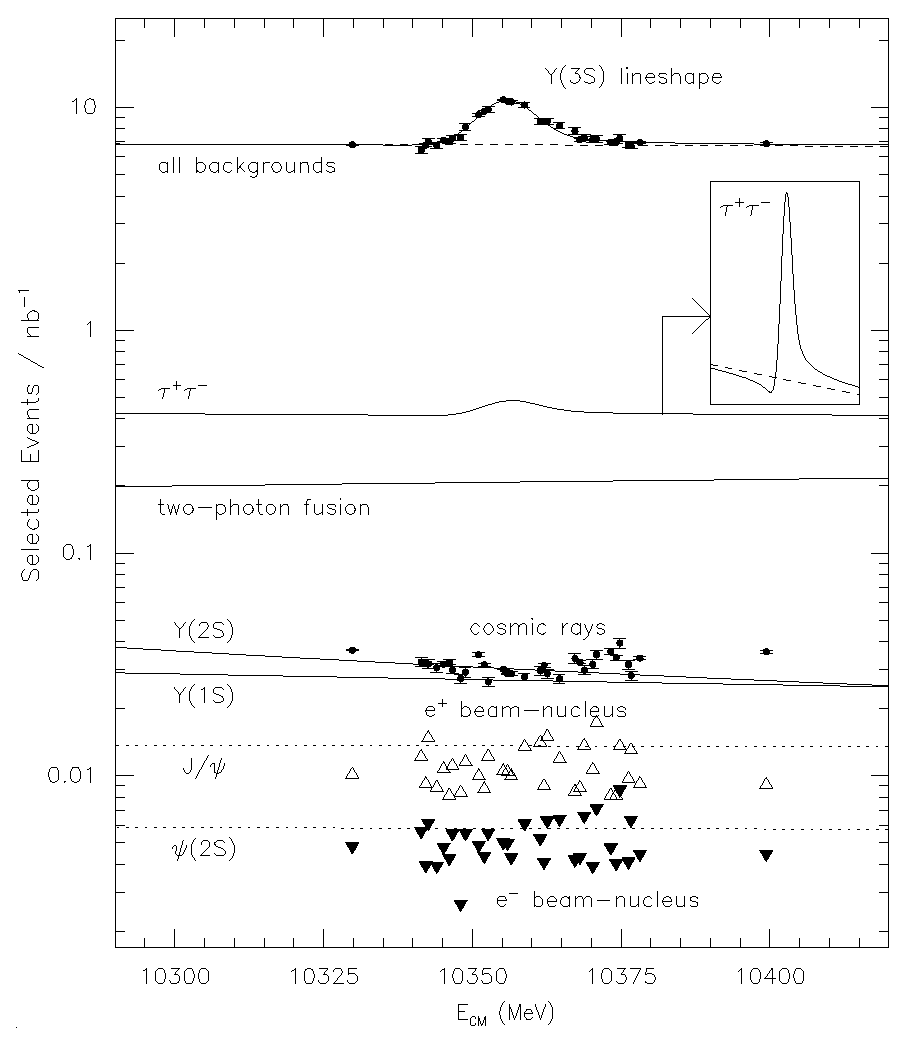
\includegraphics[width=\linewidth]{../plots/awesome}

  \caption{\label{fig:awesome} All \uthree\ backgrounds (\uone\ and
  \utwo\ backgrounds are smaller).  \vspace{0.2 cm} \\
  Lines, top to bottom: fitted lineshape, all backgrounds (dashed),
  continuum and resonance \tautau, with interference (see inset);
  two-photon fusion, which rises as $\log s$; \utwo\ and \uone\
  high-energy tails, which descend as $1/(E-M_\Upsilon)$; $J/\psi$ and
  $\psi(2S)$ tails (dotted), which are not corrected for (they
  contribute to ``two-photon''). \vspace{0.2 cm} \\
  Points, top to bottom: observed lineshape, cosmic rays (with
  statistical uncertainties), positron-induced beam-gas (open
  triangles), and electron-induced beam-gas (filled triangles).}
\end{figure}

Not all backgrounds, however, depend on beam energy as $1/s$.
Two-photon fusion, in which the incident \ee\ do not collide but emit
virtual photons which do, depends on beam energy as $\log s$.  Most of
these events have low visible energy, the sum of all charged particle
energies (measured by their track momenta, assuming pion masses) and
neutral particle energies (measured by calorimeter showers that can't
be matched to any charged tracks).  Two-photon fusion events usually
generate little visible energy in the detector because much of the
initial state energy is carried down the beampipe by one or both of
the incident beams that failed to collide.  We only accept events in
which more than 40\% of the center-of-mass energy is visible.  This
cut eliminates most of the two-photon events, which peak below 20\%
(see Figure \ref{fig:visen}).  We gauge the fraction of two-photon
events that survive this cut by fitting the three off-resonance data
points for deviations from $1/s$: correcting for high-energy tails
from \uone\ and \utwo, the fraction of two-photon events at 9 GeV is
(8.0 $\pm$ 0.5)\% (see Figure \ref{fig:backfit}).  This 8\% may
include other non-$1/s$ contributions (such as $J/\psi$ tails,
variation in continuum cut efficiency, or variation in $R$), but we
only need to know the shape of the background for the lineshape fits,
not its exact composition.

\begin{figure}[p]
  \begin{center}
    \includegraphics[width=0.9\linewidth]{../plots/proceedings_visen}
  \end{center}
  \caption{\label{fig:visen} Visible energy of off-resonance data,
    showing a large peak of two-photon background below 20\% of the
    center-of-mass energy.  The dotted line indicates the cut
    threshold and the dashed histogram shows \ups\ events on top of
    the background.}
\end{figure}

\begin{figure}[p]
  \begin{center}
    \includegraphics[width=0.9\linewidth]{../plots/proceedings_backgrounds}
  \end{center}
  \caption{\label{fig:backfit} The three off-resonance points showing
    \uone\ and \utwo\ tail corrections (corrected points are lower),
    fitted to $1/s + \log s$ (solid line).  The dashed line shows a
    pure $1/s$ fit through \uone\ off-resonance for comparison.}
\end{figure}

This visible energy cut also rejects some \tautau\ events, as these
subsequently decay into final states involving neutrinos.  However,
57\% remain after cuts, and this background is seemingly irreducible
as the final states look like hadronic events: they have two or more
low-momentum tracks without strong geometric correlations.  They are
therefore allowed to contribute to 0.57 $\times$
$\mathcal{B}_{\tau\tau}$ $\approx$ 1\% of the resonance peak.

\begin{figure}[p]
  \includegraphics[width=\linewidth]{../plots/datasets_database_dxydzcuts}
  \caption{\label{fig:cosbg} Two geometric variables used to select
    cosmic rays and beam-gas.  In each case, the histogram is all
    experimental data, and the points are a control (beamless data or
    single-beam data). \vspace{0.2 cm} \\
    (a) \dxy, the distance of closest approach of the
    closest track to the beamline, after other cosmic ray cuts (in log
    $x$ scale: 0.01 is 1 cm).  The distribution above 5 mm (dotted
    line) is well-described by no-beam data. \vspace{0.2 cm} \\
    (b) \dz, the distance of the event vertex from the
    nominal beam spot, as measured along the beamline.  Although
    beam-gas cuts reject events with \dz\ $<$ 7.5 cm (dotted line), the
    beam-gas count may be contaminated by some collision data.}
\end{figure}

Any backgrounds which vary slowly with beam energy and are
proportional to luminosity can be subsumed into the fit parameters
described above.  Cosmic rays, however, need not be proportional to
luminosity as they come from an external source.  We reject most
cosmic rays by requiring that the distance of closest approach of the
closest track to the beamline (\dxy) be less than 5 mm (a very loose
cut: \dxy\ has an RMS of 0.2 mm).  We find the number of cosmic rays
that survive hadronic cuts by applying the cuts to a control dataset
with no beams in CESR (cosmic rays only), normalized by the number of
events satisfying special cosmic ray cuts, for each energy point.
Figure \ref{fig:awesome} shows the result of this measurement for
\uthree\ data (typically 0.4\% of continuum), and Figure
\ref{fig:cosbg}-a shows \dxy\ for events that passed all other cosmic
rays cuts, for experimental and control data.

Another two backgrounds which aren't proportional to luminosity are
beam-gas events, in which one beam electron or positron collides with
a gas atom inside the beampipe, and beam-wall, in which a beam
particle collides with the wall of the beampipe.  These are suppressed
by calculating an approximate vertex for each event in Z, along the
beamline (called \dz).  Beam-gas and beam-wall events may occur
anywhere along the beamline, but beam-beam collisions must originate
within a few centimeters of the nominal beam spot.  We cut at 7.5 cm
(also loose: \dz\ has an RMS of 1.5 cm).  To count survivors, we
construct a set of beam-gas cuts and test them in a single-beam
control sample, in analogy to cosmic ray counting above (except that
cosmic rays need to be subtracted from the single-beam sample).
Figure \ref{fig:cosbg}-b shows \dz\ after other beam-gas cuts, for
experimental and control data.  Unlike cosmic rays, which are easily
distinguished from collision data and are well-represented by the
no-beam sample (\ref{fig:cosbg}-a), beam-gas cuts before \dz\ have a
large background from collision data, and the low-precision in the
single-beam sample makes it unclear how many collision events have
large \dz.  As a precaution, we subtract 50\% $\pm$ 50\% of the
estimated beam-gas background from our hadronic event count.
Beam-wall events were found to be much less common than beam-gas, and
are subsumed into this uncertainty.  As the $e^+$ and $e^-$ beams may
have different currents, we count electron-induced beam-gas
independently of positron-induced beam-gas.  (They can be
distinguished by their net Z momentum.)  Beam-gas counts are also
plotted in Figure \ref{fig:awesome}; they typically amount to 0.1\% of
the continuum.

%---------------------------------------------------------------------
%
\subsection{Hadronic Efficiency}
%
%---------------------------------------------------------------------

Now that we know we can subtract non-\ups\ events from our hadronic
event count (or cover the remainder with an uncertainty), we turn to
the issue of hadronic \ups\ decays missing from that count.  These
events may be missing because they are detected but fail our four
cuts, or, more seriously, because they fail to trigger.  The decay
$\Upsilon \to Z^* \to \nu\bar{\nu}$, which is ``hadronic'' by our
choice of definition, generates no tracks and no showers.  We need to
put a limit on invisible decays such as this, ideally one that assumes
as little as possible from a theoretical model.  This limit will
dominate the uncertainty in hadronic efficiency.

All \uone\ decays can be seen from \twotoone\ if the two tracks left
by the charged pions are sufficient to satisfy the trigger.  A pion
with more than 150 MeV of transverse momentum will generate an AXIAL
track in the trigger with (99.93 $\pm$ 0.07)\% probability
\cite{inga}.  By requiring both pions to satisfy this criterion and
selecting events from the prescaled two-track trigger, we obtain a
complete and unbaised set of \uone\ decays, though at a cost of a
factor of 20 in sample size.

The \twotoone\ events in this sample are identified by requiring the
recoil mass of the two pions
\begin{equation}
  {m_\subs{$\pi\pi$-rec}}^2 = \left(2 E_\subs{beam} - \sqrt{|\vec{p}_1|^2 + {m_\pi}^2}
  - \sqrt{|\vec{p}_2|^2 + {m_\pi}^2}\right)^2 - |\vec{p}_1 + \vec{p}_2|^2
\end{equation}
to be close to the \uone\ mass.  As can be seen in Figure
\ref{fig:recoil}-a, the \uone\ peak sits on top of a flat background
of random two-track combinations, sometimes from true \twotoone\
decays but often from other event types.  We suppress this
combinatoric background by requiring the pair of tracks to intersect
near the beam spot and to have opposite charges, but ultimately, the
remainder will need to be subtracted by a linear fit.

We first want to learn from this study how many \uone\ events are
``invisible,'' which we will take to mean how many fail to generate
one AXIAL track and one CBLO (150 MeV cluster) in the trigger.  This
is a necessary condition for the analysis trigger, so any event that
fails this simple criterion will fail the exact trigger criteria
described in Equation \ref{eqn:trig}.  We fit the recoil mass peak to
a double Gaussian (Figure \ref{fig:recoil}-a) and use the same mean,
sigmas, and area ratio in a fit to the invisible events (Figure
\ref{fig:recoil}-b).  The ratio of these two is (0.67 $\pm$ 0.62)\%,
so the probability for an \uone\ to be visible to the trigger is
(99.33 $\pm$ 0.62)\%.

The hadronic efficiency of our cuts can be more precisely determined
because we do not need to use as small a set of \twotoone\ events.
Instead of only considering events from the prescaled two-track
trigger, we can use events from an unprescaled trigger which requires
three AXIAL tracks and one CBLO.  This sample is called low-bias (see
Figure \ref{fig:recoil}-c for a recoil mass plot) because the \uone\
must supply one AXIAL track and one CBLO.  (In other words, it must be
``visible.'')  We apply our hadronic cuts, excluding the two pions, to
this sample and count \#pass/(\#pass $+$ \#fail) by subtracting scaled
sideband events (\mpprec\ $\in$ (9.441, 9.454) $\cup$ (9.472, 9.480)
GeV) from signal events (9.454 $<$ \mpprec\ $<$ 9.472 GeV).  Figure
\ref{fig:recoil}-d shows the recoil mass of events that failed the
cuts.  This fraction, which includes $\Upsilon(1S) \to e^+e^-$,
$\mu^+\mu^-$, and $\tau^+\tau^-$, is (92.58 $\pm$ 0.13)\%.  Correcting
for leptonic modes, the cut efficiency for hadronic decays is (98.32
$\pm$ 0.21)\%.

We repeated this procedure for \twotoone\ Monte Carlo, and obtained a
(98.54 $\pm$ 0.22)\% hadronic cut efficiency, in good agreement with
the data.  We also simulated $e^+e^- \to \Upsilon(1S) \to$ hadronic
modes, in which we found a (98.68 $\pm$ 0.04)\% efficiency: also in
good agreement.  This shows that the $\gamma$ = 1.003 boost of the
\uone\ in \twotoone\ and track/shower confusion from the pions account
for a 1.0014 $\pm$ 0.0022 correction.  Thus the unboosted, hadronic
\uone\ cut efficiency is (98.46 $\pm$ 0.30)\%.

Distributions of the four variables used in our cuts are presented in
Figure \ref{fig:4var}, after combinatric background subtraction.
Monte Carlo (\twotoone) is overlaid for comparison.

In general, our analysis trigger requires more than one AXIAL track
and one CBLO.  The trigger efficiency, after this ``visible''
condition and our hadronic cuts, is 99.87\% in Monte Carlo.  A
comparison of AXIAL, STEREO, CBLO, and CBMD distributions in data and
Monte Carlo indicate that the simulation can be trusted, at the very
least within 100\% of the predicted effect (Figure \ref{fig:mctrig}),
so we will assign it a systematic error of 0.13\%.  The \uone\
hadronic efficiency is (97.66 $\pm$ 0.70)\%, the product of these
three cumulative contributions (listed in Table \ref{tab:fityields}).

\begin{figure}[t]
  \begin{center}
    \Large $\pi^+\pi^-$ recoil mass in GeV
  \end{center}

  \vspace{-1.8 cm}
  \begin{center}
    \includegraphics[width=0.9\linewidth]{../plots/proceedings_fityields2}
  \end{center}
  \caption{\label{fig:recoil} Recoil mass of $\pi^+\pi^-$ in (a) the
    unbiased sample (all \ups\ decays are present), (b) the unbiased
    sample for invisible decays (no AXIAL tracks or no 150 MeV
    clusters), (c) the low-bias sample (\ups\ must be visible), and
    (d) the low-bias sample failing hadronic cuts.  Most of the \uone\
    decays in (d) are lepton pairs.}
\end{figure}

\begin{table}[t]
  \begin{center}
    \begin{tabular}{r l c c}
      \hline \hline & Criterion & Efficiency \\ \hline
      1. & Visible to trigger: $\ge$1 AXIAL track and $\ge$ 1 CBLO (150 MeV cluster) & (99.33 $\pm$ 0.62)\% \\
         & Passed all cuts (assuming visible \uone)                                  & (92.58 $\pm$ 0.13)\% \\
         & Passed all cuts (assuming visible hadronic \uone)                         & (98.32 $\pm$ 0.21)\% \\
      2. & Passed all cuts without boost/track confusion (assuming the above)        & (98.46 $\pm$ 0.30)\% \\
      3. & Passed trigger (Equation \ref{eqn:trig})                                  & (99.87 $\pm$ 0.13)\% \\ \hline
         & \uone\ hadronic efficiency (product of 1, 2, and 3)                       & (97.66 $\pm$ 0.70)\% \\ \hline \hline
%%       largest track momentum ($\times c$) $<$ 80\% of beam energy & (94.62 $\pm$ 0.07)\% & \\
%%       visible energy $>$ 40\% center-of-mass energy & (98.76 $\pm$ 0.10)\% & \\
%%       $|d_{XY}|$ $<$ 5 mm & (99.94 $\pm$ 0.02)\% & \\
%%       $|d_{Z}|$ $<$ 7.5 cm  & (99.12 $\pm$ 0.04)\% & \\ \hline \hline
    \end{tabular}
  \end{center}
  \caption{\label{tab:fityields} Summary of cut efficiency
    measurement for \uone.}
\end{table}

\begin{figure}[p]
  \vspace{3 cm}
  \begin{center}
    \includegraphics[width=0.9\linewidth]{../plots/proceedings_cuts3}
  \end{center}
  \caption{\label{fig:4var} The four hadronic cuts, as seen in
    \twotoone\ decays.  Points are data and histograms are Monte
    Carlo; dotted lines are cut thresholds.  (a) Biggest track
    momentum $<$ 80\% beam energy (cross-hatched histogram is \ee,
    \mm\ Monte Carlo), (b) visible energy $>$ 40\% expected
    center-of-mass energy, (c) $|d_{XY}|$ $<$ 5 mm, and (d) $|d_Z|$
    $<$ 7.5 cm.}
\end{figure}

\begin{figure}[p]
  \vspace{3 cm}
  \begin{center}
    \includegraphics[width=0.9\linewidth]{../plots/trigger_lowlevel_1s_2}
  \end{center}
  \caption{\label{fig:mctrig} Trigger variables as seen in hadronic
    data (points) and in Monte Carlo (histogram).  (a) Number of AXIAL
    tracks, (b) STEREO tracks, (c) CBLO (150 MeV clusters), and (d)
    CBMD (750 MeV clusters).  The analysis trigger decision is derived
    from these variables using Equation \ref{eqn:trig} (the lower
    limits are indicated by dotted lines).  Data have been
    continuum-subtracted, cosmic-ray and beam-gas-subtracted, and the
    leptonic modes have been subtracted using Monte Carlo.}
\end{figure}

The \utwo\ and \uthree\ differ from the \uone\ in their ability to
cascade into lower \ups\ states, which can subsequently decay into
\ee\ and \mm.  These are hadronic decays, but they will fail our cuts
because they contain high-momentum tracks.  We generated \utwo\ and
\uthree\ Monte Carlo to determine the efficiencies of these ``cascade
to lepton'' events: (0.69 $\pm$ 0.22)\% for \utwo\ and (0.38 $\pm$
0.19)\% for \uthree.

To correct for these inefficiencies, we also need to know the
branching fractions for cascades to leptons
($\mathcal{B}_\subs{cas-lep}$).  We measured this in data by rejecting
Bhabha background with a largest shower $<$ 70\% of beam energy cut
and counting the fraction of continuum-subtracted events with two
large tracks ($>$ 70\% of beam energy).  This is the fraction of \ups\
decays with any muon pair in the final state; we subtract
$\mathcal{B}_{\mu\mu}$ and multiply by two for
$\mathcal{B}_\subs{cas-lep}(2S)$ = (1.54 $\pm$ 0.36)\% and
$\mathcal{B}_\subs{cas-lep}(3S)$ = (1.44 $\pm$ 0.48)\%.

Thus the Monte Carlo's prediction for \utwo\ and \uthree\ hadronic
efficiency is
\begin{eqnarray}
  \epsilon_{MC} &=& (\mathcal{B}_\subs{cas-lep}) \, \epsilon_\subs{cas-lep, MC}
  + (1 - \mathcal{B}_\subs{cas-lep}) \, \epsilon_\subs{all other modes, MC} \\
  & & \nonumber \\
  \epsilon_{MC}(2S) &=& (0.0154) \, 0.69\% + (1 - 0.0154) \, 98.45\% = \mbox{(96.94 $\pm$ 0.40)\%} \nonumber \\
  \epsilon_{MC}(3S) &=& (0.0144) \, 0.38\% + (1 - 0.0144) \, 98.45\% = \mbox{(97.04 $\pm$ 0.50)\%.} \nonumber
\end{eqnarray}
We use the Monte Carlo's predictions to scale the \uone\ efficiency
measurement to the \utwo\ and \uthree:
\begin{eqnarray}
  \epsilon(nS) &=& \epsilon(1S) \times \left(\epsilon_{MC}(nS) / \epsilon_{MC}(1S)\right) \\
  & & \nonumber \\
  \epsilon(1S) &=& \mbox{(97.66 $\pm$ 0.70)\%} \nonumber \\
  \epsilon(2S) &=& \mbox{(97.66 $\pm$ 0.70)\%} \times \left(\frac{\mbox{(96.94 $\pm$ 0.40)\%}}{\mbox{(98.68 $\pm$ 0.04)\%}}\right) = \mbox{(95.94 $\pm$ 0.81)\%} \nonumber \\
  \epsilon(3S) &=& \mbox{(97.66 $\pm$ 0.70)\%} \times \left(\frac{\mbox{(97.04 $\pm$ 0.50)\%}}{\mbox{(98.68 $\pm$ 0.04)\%}}\right) = \mbox{(96.04 $\pm$ 0.86)\%.} \nonumber
\end{eqnarray}
Thus, the \utwo\ and \uthree\ hadronic efficiencies are (95.94 $\pm$
0.81)\% and (96.04 $\pm$ 0.86)\%, respectively.

%---------------------------------------------------------------------
%
\subsection{Luminosity}
%
%---------------------------------------------------------------------

For each beam energy, we can now count hadronic \ups\ decays, subtract
non-\ups\ backgrounds from this count, and correct it for missing
\ups\ events.  All that remains is to remove the effects of variable
run lengths by converting this number into a cross-section: we need to
measure the integrated luminosity at each energy point.  We have two
concerns: the first is to determine the integrated luminosity of each
energy point up to a single constant, so that observed lineshapes are
undistorted.  We will call these the relative luminosities and measure
them by counting Gamgam events at each energy.  The second concern is
to determine the last constant, the absolute luminosity, turning a
number of Gamgams into nb\inv\ and setting the scale for all three
\gee\ measurements.

Gamgam events ($e^+e^- \to \gamma\gamma$) have a distinct signature,
two large, back-to-back showers, so backgrounds are not an issue above
our level of consideration (0.1\%).  Also, we do not need to know the
efficiency of our cuts for a relative luminosity measurement.  We
require there to be no tracks in the drift chamber, two large ($>$
70\% of beam energy) showers in the calorimeter which are back-to-back
in $\phi$ (the polar angle around the beamline; we require $|\sin
\phi_1 - \phi_2|$ $<$ 0.04 to avoid the nearly back-to-back showers
from \ee), and back-to-back in $\theta$ (the azimuthal angle; we
require $|\cot\theta_1 + \cot\theta_2|$ $<$ 0.1, as the calorimeter
has a barrel geometry and crystal elements are equally spaced in
$\cot\theta$).  We also restrict ($\theta_1$, $\theta_2$) to be far
from the edge of the calorimeter barrel ($\min(|\cot\theta_1|,
|\cot\theta_2|) < 1.18$ and $\max(|\cot\theta_1|, |\cot\theta_2|) <
1.28$) and far from the center ($\min(|\cot\theta_1|, |\cot\theta_2|)
> 0.05$ and $\max(|\cot\theta_1|, |\cot\theta_2|) > 0.15$).  At the
edge, showers may be clipped, and at the center, the trigger is
inefficient.

Since Gamgam events have no tracks, they rely on the back-to-back 1.5
GeV-cluster trigger.  This trigger accepts events with two high-energy
clusters which are moderately back-to-back in $\phi$ (our cut is much
tighter) and on opposite sides of the detector in $\theta$.  Near the
center of the detector, measurement error sometimes puts both energy
clusters on the same side of the detector, and the trigger is
inefficient.  We cut this region out.  There are three other regions
where the trigger is inefficient: some calorimeter trigger tiles were
unresponsive for part of \ups\ data-taking.  We also cut these regions
out (for all data).  After all cuts, the trigger efficiency is 99.7\%
at every energy point; this was measured by selecting Bhabhas with
another trigger and asking how often Gamgam's trigger is satisfied.
All deviations from 99.7\% efficiency are statistical (with
$\sim$0.2\% precision in each run).  Therefore, we need not be
concerned that hadronic events are counted while Gamgams fail to
trigger, which would artificially raise the cross-section measurement.

We might also ask the inverse question: can Gamgams continue to be
counted while the drift chamber fails to trigger, artificially
lowering the cross-section measurement?  In principle, it could: the
drift chamber may lose high voltage and therefore lose sensitivity to
charged particles.  In such cases, the CLEO operator immediately ends
the run and resets the machine, but it is a good idea to find out how
common this problem is.  We checked for it by searching for Bhabhas
without tracks, that is, Bhabhas identified by the calorimeter ($0.04
< |\sin \phi_1 - \phi_2| < 0.25$, using the Gamgam trigger) with no
tracks in the drift chamber.  In good runs, at most 0.3\% of Bhabhas
have no tracks (Gamgam might be a background), though twenty-five runs
in the \ups\ data were found with a period of drift chamber
insensitivity.  Each of them lasted only a few minutes before the
machine was reset.  These runs were excluded from the lineshape fits.

In the three off-resonance data points, where Bhabha events have no
backgrounds from \ups, the Gamgam/Bhabha ratio is 0.0793 $\pm$ 0.0002,
0.0792 $\pm$ 0.0001, and 0.0793 $\pm$ 0.0002, all in statistical
agreement and very precise (0.2\%).  This gives us confidence that the
relative luminosity measurement is stable.

The absolute luminosity measurement, to convert Gamgam counts into
nb\inv, has been extensively studied elsewhere \cite{lumi}.  This
study selects Bhabhas, Mupairs, and Gamgams, simulates a given
integrated luminosity with Monte Carlo, and attempts to determine the
absolute normalization of each.  The three measurements yield $x$
nb\inv, $y$ nb\inv, and $z$ nb\inv\ for all off-resonance data and we
count $N$ Gamgam events in the same data.  The factor $<x,y,z>/N$
converts any Gamgam count into nb\inv, but this factor has an error of
$Q$\% of itself, as the three measurements differ beyond their
uncertainties with a $\chi^2$ of $P$.

%---------------------------------------------------------------------
%
\section{Fitting}
%
%---------------------------------------------------------------------

For each resonance lineshape fit, the background level $\sigma_b$ is
allowed to float: the $1/s + \log s$ background shape is only
extrapolated 50 MeV or so within an \ups\ lineshape.  The Breit-Wigner
area (\gee) also floats, as does the beam energy spread $\Delta E$.
The peak position of each weekly scan (12 for \uone, 6 for \utwo, and
7 for \uthree) also floats in the fit.  By this, we mean that data
from one week can slide up and down in beam energy independently of
data from another week, while the theoretical lineshape is fixed at
the known \ups\ mass.

The peak fit function is a convolution of a Breit-Wigner, a Gaussian,
and an initial-state radiation tail, with an interference term between
the Breit-Wigner and the continuum background.  The \ups\ has a 10\%
branching fraction to $q\bar{q}$, and $e^+e^- \to q\bar{q}$ is the
primary component of the continuum.  In principle, the observed
cross-section is not the sum of these two, but is proportional to the
squared sum of their amplitudes:
\begin{eqnarray}
  \sigma(e^+e^- \to X \to q\bar{q}) &\propto& |\mathcal{M}(e^+e^- \to q\bar{q}) + \mathcal{M}(e^+e^- \to \Upsilon \to q\bar{q})|^2 \\
  &\propto& |\mathcal{M}(e^+e^- \to q\bar{q})|^2 + |\mathcal{M}(e^+e^- \to \Upsilon \to q\bar{q})|^2 + \nonumber \\
  & & \mbox{\hspace{1.5 cm}} 2 \, \mathrm{Re\:} \mathcal{M}(e^+e^- \to q\bar{q})^* \mathcal{M}(e^+e^- \to \Upsilon \to q\bar{q}) \mbox{.}
\end{eqnarray}
The last term is the interference term, and it distorts the \ups\
lineshape by causing a deficit of events below the \ups\ mass and an
excess above it.  The data, however, are not statistically sensitive
to this effect.  (The interference term, at its maximum, is about a
factor of 70 smaller than the peak at its maximum.)

As previously mentioned, 57\% of $\Upsilon \to \tau^+\tau^-$ survive
hadronic cuts, so these are added as a contribution to the fit
function.  These events have the same distribution as hadrons, except
for an interference term which is larger by a factor of 10 (see the
inset in Figure \ref{fig:awesome}).

The background has the $1/s + \log s$ shape described in Section
\ref{sec:back}, plus tails from \uone\ and \utwo.

The \uone, \utwo, and \uthree\ lineshape fits, with statistical
uncertainties of 0.64\%, 1.57\%, 2.09\%, and reduced $\chi^2$ of 1.19,
0.95, 0.90, respectively (Table \ref{tab:fits}), are presented in
Figure \ref{fig:fits} with pull distributions in Figures
\ref{fig:pull1}, \ref{fig:pull2}, and \ref{fig:pull3}.  The
statistical uncertainties are dominated by Gamgam counting.  The
\uone\ fit $\chi^2$ is too large: it corresponds to a confidence level
of 0.4\%, and suggests that the uncertainties assigned to our points
is 10\% too small, which could be accomodated by an additional
uncertainty of 0.3\%.

Systematic uncertainties from varying each fixed parameter are listed
in Table \ref{tab:lineshape}.  These fits assume zero uncertainty in
the beam energy measurement, a situation which we will now remedy.

\begin{table}
  \begin{center}
    \begin{tabular}{l c c c}
      \hline\hline
      & \uone & \utwo & \uthree \\\hline
      $\chi^2/$\#degrees of freedom & $\displaystyle \frac{508.7}{443-15}$ = 1.19 & $\displaystyle \frac{112.3}{127-9}$ = 0.95 & $\displaystyle \frac{412.1}{469-10}$ = 0.90 \\
      Confidence level & 0.4\% & 63\% & 94\% \\
      $\int \sigma(e^+e^- \to \Upsilon) \, dE$ (MeV nbish) & 13.697 $\pm$ 0.055 & 5.712 $\pm$ 0.045 & 3.639 $\pm$ 0.029 \\
      Statistical uncertainty & 0.64\% & 1.57\% & 2.09\% \\ \hline\hline
    \end{tabular}
  \end{center}
  \caption{\label{tab:fits} Fit results.}
\end{table}

\begin{table}
  \begin{center}
    \begin{tabular}{l c c c}
      \hline\hline
      & \uone & \utwo & \uthree \\\hline
      Uncertainty in $\Gamma$                           & 0.005\% & 0.02\%  & 0.03\% \\
      Interference term ($\mathcal{B}_{\mu\mu}$, $R$)   & 0.02\%  & 0.02\%  & 0.002\% \\
      Two-photon fraction                               & 0.002\% & 0.002\% & 0.001\% \\
      Initial-state radiation tail (0.1\% theory error) & 0.05\%  & 0.05\%  & 0.04\% \\\hline
      Total (in quadrature)                             & 0.05\%  & 0.06\%  & 0.05\% \\\hline\hline
    \end{tabular}
  \end{center}
  \caption{\label{tab:lineshape} Systematic uncertainties in the
    shape of the fit function.}
\end{table}

\begin{figure}[p]
  \includegraphics[width=\linewidth]{../fit_results/effcor_allfit_comb}
  \caption{\label{fig:fits} Best-fit to the (a) \uone\ lineshape, (b)
    \utwo\ lineshape, and (c) \uthree\ lineshape.  Measurements at the
    same beam energy have been combined in this plot, but not in the
    fit.}
\end{figure}

\begin{figure}[p]
  \includegraphics[width=\linewidth]{../fit_results/effcor2_1pull}
  \caption{\label{fig:pull1} Pull distributions ((observed $-$
    fit)/uncertainty) for the \uone\ fit: (a) versus energy, (b)
    versus date of measurement, and (c) as a histogram.}
\end{figure}

\begin{figure}[p]
  \includegraphics[width=\linewidth]{../fit_results/effcor2_2pull}
  \caption{\label{fig:pull2} Pull distributions ((observed $-$
    fit)/uncertainty) for the \utwo\ fit: (a) versus energy, (b)
    versus date of measurement, and (c) as a histogram.}
\end{figure}

\begin{figure}[p]
  \includegraphics[width=\linewidth]{../fit_results/effcor2_3pull}
  \caption{\label{fig:pull3} Pull distributions ((observed $-$
    fit)/uncertainty) for the \uthree\ fit: (a) versus energy, (b)
    versus date of measurement, and (c) as a histogram.}
\end{figure}

%---------------------------------------------------------------------
%
\section{Beam Energy Uncertainty}
%
%---------------------------------------------------------------------

We minimized our sensitivity to uncertainties in the beam energy
measurement by collecting data in small, independent scans, and by
alternating measurements above and below the \ups\ mass.  To measure
this uncertainty, most weekly scans included two cross-section
measurements at the same beam energy, usually near the beginning and
end of the scan and at a point where the lineshape has a high
derivative.  (Some scans included more than one repeated measurement.)
If the beam energy calibration does not fluctuate between the two
measurements, the hadronic cross-sections should be statistically
consistent.  If it fluctuates by a large amount, we would see a
different hadronic cross-section, and can divide this difference by
the derivative of the fitted lineshape to measure the shift in beam
energy calibration.  If the beam energy fluctuates rapidly, many times
during a single cross-section measurement, this contributes to $\Delta
E$ and is not measurable (or relevant).  Note that the calibration
shifts under consideration here would take place during a weekly scan,
not between them, so they can distort the lineshape and add to
$\chi^2$.

We converted thirty pairs of repeated measurements into beam energy
calibration shifts, and plotted them in Figure \ref{fig:miscal} as a
function of time between the end of the early and the beginning of the
late measurement.  As there is no evidence of any calibration shift,
we constructed an upper limit the following way: we define
\begin{equation}
  -\mbox{log likelihood}(\sigma_E) = \sum_{i=1}^{30} -\ln \left(\frac{1}
  {\sqrt{2\pi ({\sigma_{s_i}}^2 + {\sigma_E}^2)}} \exp\left(
  -s_i^2 / 2 / ({\sigma_{s_i}}^2 + {\sigma_E}^2) \right) \right)
\end{equation}
where $s_i \pm \sigma_{s_i}$ are the calibration shift measurements
plotted in Figure \ref{fig:miscal}, and $\sigma_E$ is an assumed
uncertainty in beam energy.  When $\sigma_E$ is zero, $-$log
likelihood is $-$0.71.  To raise $-$log likelihood by 0.5, we need a
$\sigma_E$ of 0.05 MeV.

\begin{figure}[t]
  \begin{center}
    \includegraphics[width=0.9\linewidth]{../plots/proceedings_miscal}
  \end{center}
  \caption{\label{fig:miscal} Beam energy calibration shifts, as
    determined from thirty pairs of repeated cross-section
    measurements (plotted versus time).}
\end{figure}

To find out what this $\sigma_E$ implies for the lineshape fits, we
simulate data-taking and fitting with a toy Monte Carlo that samples
the same data points and fits to the same fit function.  The hadronic
cross-sections are simulated using the fitted lineshape as a template,
and then the beam energy is randomly fluctuated (jittered) with an RMS
of $\sigma_E$ = 0.05 MeV.  In an ensemble of energy jitters for a
fixed dataset, \gee\ differs from the no-jitter case by a root mean
square deviation of 0.07\%, 0.13\%, 0.27\% for the three resonances
and $\chi^2$ differs by 4.2, 1.4, and 3.0 [very rough: not the real
calculation].  These results are stable when new datasets are
simulated.  We therefore assign a 0.07\%, 0.13\%, 0.27\% systematic
uncertainty to \gee\ due to beam-energy uncertainty, and note that
this effect cannot account for the large $\chi^2$ observed in the real
\uone\ fit.

%---------------------------------------------------------------------
%
\section{Conclusions}
%
%---------------------------------------------------------------------

Measured values of \gee\ and all systematic uncertainties are listed
in Table \ref{tab:finalgee}.  Ratios of \gee\ (for which absolute
luminosity and some efficiency systematics cancel) are listed in Table
\ref{tab:ratios}, and $\Gamma_{ee}\Gamma_\subs{had}/\Gamma_\subs{tot}$ in
Table \ref{tab:geehadtot}.  Statistical uncertainties include
background subtractions and uncertainties in relative luminosity
measurements (Gamgam counting statistics).  

We plan to improve this measurement by replacing Gamgams with Bhabhas
as a measure of relative luminosity, reducing the statistcal
uncertainties by a factor of 3.55, but possibly introducing new
systematic errors.

\begin{table}[p]
  \begin{center}
    \begin{tabular}{l c c c}
      \hline\hline
      Contribution & \mbox{\hspace{1 cm}} \uone\ \mbox{\hspace{1 cm}} & \mbox{\hspace{1 cm}} \utwo\ \mbox{\hspace{1 cm}} & \mbox{\hspace{1 cm}} \uthree\ \mbox{\hspace{1 cm}} \\\hline
      Statistical                         & 0.64\% & 1.57\% & 2.09\% \\
      Hadronic efficiency                 & 0.70\% & 0.81\% & 0.86\% \\
      $(1 - 3\mathcal{B}_{\mu\mu})$       & 0.24\% & 0.27\% & 0.40\% \\
      Luminosity calibration              & 1.8\% & 1.8\% & 1.8\% \\
      Shape of the fit function           & 0.05\% & 0.06\% & 0.05\% \\
      Beam-energy uncertainty             & 0.07\% & 0.13\% & 0.27\% \\\hline
%%      Result (MeV nbish, later keV)       & 13.70 $\pm$ 0.28 & 5.71 $\pm$ 0.15 & 3.64 $\pm$ 0.11 \\
%% (1-3Bmm) = 0.9253 0.9391 0.9283
      Result (MeV nbish, later keV)       & 14.81 $\pm$ 0.30 & 6.08 $\pm$ 0.16 & 3.92 $\pm$ 0.12 \\
      Fractional uncertainty              & 2.05\% & 2.54\% & 2.92\% \\\hline\hline    
    \end{tabular}
  \end{center}
  \caption{\label{tab:finalgee} Values and uncertainties in \gee.}
\end{table}

\begin{table}[p]
  \begin{center}
    \begin{tabular}{l c c c}
      \hline\hline
      Contribution & \mbox{\hspace{0.5 cm}} \utwo/\uone\ \mbox{\hspace{0.5 cm}} & \mbox{\hspace{0.5 cm}} \uthree/\uone\ \mbox{\hspace{0.5 cm}} & \mbox{\hspace{0.5 cm}} \uthree/\utwo\ \mbox{\hspace{0.5 cm}} \\\hline
      Statistical                       & 1.70\% & 2.19\% & 2.61\% \\
      Hadronic efficiency               & 0.40\% & 0.50\% & 0.64\% \\
      $(1 - 3\mathcal{B}_{\mu\mu})$     & 0.36\% & 0.47\% & 0.48\% \\
      Luminosity calibration            & 0 & 0 & 0 \\
      Shape of the fit function         & 0.08\% & 0.07\% & 0.08\% \\
      Beam-energy uncertainty           & 0.15\% & 0.28\% & 0.30\% \\\hline
      Result                            & 0.4105 $\pm$ 0.0073 & 0.2647 $\pm$ 0.0061 & 0.645 $\pm$ 0.018 \\
      Fractional uncertainty            & 1.79\% & 2.30\% & 2.73\% \\\hline\hline    
    \end{tabular}
  \end{center}
  \caption{\label{tab:ratios} Values and uncertainties in ratios of \gee.}
\end{table}

\begin{table}[p]
  \begin{center}
    \begin{tabular}{l c c c}
      \hline\hline
      Contribution & \mbox{\hspace{1 cm}} \uone\ \mbox{\hspace{1 cm}} & \mbox{\hspace{1 cm}}\utwo\ \mbox{\hspace{1 cm}} & \mbox{\hspace{1 cm}} \uthree\ \mbox{\hspace{1 cm}} \\\hline
      Statistical                             & 0.64\% & 1.57\% & 2.09\% \\
      Hadronic efficiency                     & 0.70\% & 0.81\% & 0.86\% \\
      Uncertainty in $\mathcal{B}_{\tau\tau}$ & 0.09\% & 0.98\% & 1.45\% \\
      Luminosity Calibration                  & 1.8\% & 1.8\% & 1.8\% \\
      Shape of the fit function               & 0.05\% & 0.06\% & 0.05\% \\
      Beam-energy uncertainty                 & 0.07\% & 0.13\% & 0.27\% \\\hline
      Result (MeV nbish, later keV)           & 13.68 $\pm$ 0.28 & 5.73 $\pm$ 0.16 & 3.64 $\pm$ 0.12 \\
      Fractional uncertainty                  & 2.04\% & 2.71\% & 3.23\% \\\hline\hline    
    \end{tabular}
  \end{center}
  \caption{\label{tab:geehadtot} Values and uncertainties in
    $\Gamma_{ee}\Gamma_\subs{had}/\Gamma_\subs{tot}$.  We have not
    assumed Lepton Universality in this Table.}
\end{table}

%---------------------------------------------------------------------
%
\section{Acknowledgements}
%
%---------------------------------------------------------------------

We gratefully acknowledge the effort of the CESR staff in providing us
with excellent luminosity and running conditions.  This work was
supported by the National Science Foundation, and the U.S. Department
of Energy.  [Ritchie, Karl, Istvan, Surik, Rich Galik, Brian, Jean,
Steve Dytman, and Christine Davies\ldots]

\vfill

\section{Not a part of the paper}

Uncertainties:
\begin{tabular}{l c c c c}
  & \mbox{\hspace{0.25 cm}} \uone\ \mbox{\hspace{0.25 cm}} & \mbox{\hspace{0.25 cm}} \utwo\ \mbox{\hspace{0.25 cm}} & \mbox{\hspace{0.25 cm}} \uthree\ \mbox{\hspace{0.25 cm}}  & \mbox{\hspace{0.25 cm}} \utwo/\uone\ \mbox{\hspace{0.25 cm}} \\\hline
  CLEO '84 & & & 9.4\% \\
  Novosibirsk '96 & 3.3\% & 6.4\% & & 4.7\% \\
  PDG average & 2.2\% & 4.1\% & 9.4\% & \\
  This analysis & 2.1\% & 2.5\% & 2.9\% & 1.8\%
\end{tabular}

%---------------------------------------------------------------------
%
%\section{Figures}
%
%---------------------------------------------------------------------

%% \ref{fig:diagrams}
%% \ref{fig:fits}
%% \ref{fig:awesome}
%% \ref{fig:visen}
%% \ref{fig:cosbg}
%% \ref{fig:4var}
%% \ref{fig:recoil}
%% \ref{fig:pull1}
%% \ref{fig:pull2}
%% \ref{fig:pull3}
%% \ref{fit:miscal}

%% \ref{tab:eff}
%% \ref{tab:lineshape}
%% \ref{tab:finalgee}
%% \ref{tab:geehadtot}

%---------------------------------------------------------------------
%
%\section{Bibliography}
%
%---------------------------------------------------------------------
\def\endpoint{;~~}
\def\Journal#1&#2&#3(#4){#1{\bf #2}, #3 (#4)}
\def\NIM{Nucl. Instr. and Meth. }
\def\NIMA{Nucl. Instr. and Meth. A }
\def\NPB{Nucl. Phys. B }
\def\PLB{Phys. Lett. B }
\def\PRL{Phys. Rev. Lett. }
\def\PRD{Phys. Rev. D }
\newpage
\begin{thebibliography}{99}

\bibitem{cleo3det} CLEO Collaboration, CLNS-94-1277; D.\ Peterson \etal, {\Journal\NIMA&478&142(2002)}

\bibitem{kb} Primer on Onium Widths, but a copy with interference; K.\ Berkelman, ???

\bibitem{davies} Christine Davies

\bibitem{kf} Kuriev and Fadin

\bibitem{lumi} Luminosity CBX

\bibitem{inga} Inga's DR trigger study

\bibitem{XXX} Much more to come!

\end{thebibliography}

\end{document}




%% \begin{table}
%% \begin{center}
%% \caption{Features of Set A and Set B.}
%% \smallskip
%% \begin{tabular}{lcc}
%% \hline
%% Quantity & ~~~~Set A & ~~~~Set B\cr 
%% \hline\hline
%% Fraction of total \nbb\     & 55\%    & 45\%  \cr
%% Track Resolution            &         &       \cr
%% \hfil{`A' Coefficient}      & 0.0055  & 0.0044\cr
%% \hfil{`B' Coefficient ($\gev^{-1}$)}      & 0.0011  & 0.0010\cr
%% $K^+\pi^-$ Mode             &         &       \cr
%% \hfil{$\sigma_{\mb}$ (\mev)}  & 2.7     & 2.7   \cr
%% \hfil{$\sigma_{\de}$(\mev)}   & 22      & 19    \cr
%% \hfil{Efficiency}           & 38\%    & 45\%  \cr
%% $K^+\pi^0$ Mode             &         &       \cr
%% \hfil{$\sigma_{\mb}$ (\mev)}  & 3.1     & 3.1   \cr
%% \hfil{$\sigma_{\de}$(\mev)}   & 31      & 31    \cr
%% \hfil{Efficiency}           & 33\%    & 35\%  \cr
%% $\pi^0\pi^0$ Mode\footnote{Resolutions are given as average of low-side and high-side half-resolutions.}           &         &       \cr
%% \hfil{$\sigma_{\mb}$ (\mev)}  & 3.6     & 3.6  \cr
%% \hfil{$\sigma_{\de}$(\mev)}   & 43      & 43    \cr
%% \hfil{Efficiency}           & 22\%    & 22\%  \cr
%% \hline
%% \end{tabular}
%% \label{tab:oldnew}
%% \end{center}
%% \end{table}

%% \bibitem{fleischeretal} 
%% Y.-Y. Keum, H.-N. Li, and A.I. Sanda, arXiv:hep-ph/0201103; 
%% M. Neubert,                  {JHEP} {\bf 9902} (1999) 014;
%% M. Neubert and J.L. Rosner,  {\Journal\PRL&81&5076(1998)};

%% \bibitem{cleo3det}     CLEO Collaboration, CLNS-94-1277; D. Peterson \etal, {\Journal\NIMA&478&142(2002)}

%% \bibitem{pdg} Particle Data Group, {\Journal\PRD&66&010001(2002)}.\label{ref:pdg}
